\chapter{méthodes (MIC 2010)}

J'ai utilisé la base de donnée présentée dans la partie\ref{lab:bdd} pour évaluer les performances des techniques de correction du mouvement respiratoire présentés dans le chapitre \ref{lab:corrMvt}. 

Les techniques de correction du mouvement implémentées sont les suivantes :

\begin{enumerate}
 \item Correction pendant la reconstruction par modification de la matrice système (voir section \ref{lab:corrMatSyst})
 \item Correction post-reconstruction par recalage des images prises à différents instants du cycle (voir section \ref{lab:corrPostRecon})
\end{enumerate}

Elles sont comparées avec les images non Corrigées et des images statiques (qui représentent une correction parfaite).

Dans le cas présent, l'objectif est d'évaluer les performances des techniques de correction du mouvement sur la détection des lésions de faible contraste/faible diamètre. Pour cela, les performances d'un système de détection automatique seront comparées sur les différents types d'images.

\section{Système CAD}

Le système CAD utilise des informations fréquentielles obtenue par décomposition non décimée des images en ondelettes Biorthogonale 4.4. Ces données sont utilisées par le système de classification basé sur un SVM travaillant voxel par voxel. Une étape de réduction des faux positifs est ajoutée par la suite.
\'Etant donné le faible nombre de tumeurs présentes dans les organes considérés, la base d'apprentissage est générée à partir des images utilisées pour la base de test. 

\subsection{Vecteur de Caractéristiques}

Nous avons choisi d’utiliser une décomposition en ondelettes 3D par banc de filtres. Dans le cas tridimensionnel, la décomposition par banc de filtre est résumé par la Figure \ref{fig:ondelettes}. L’image de départ est filtrée séparément dans les trois directions de l’espace par un filtre fréquentiel passe-haut correspondant à la fonction d’ondelettes (noté $H$) et passe-bas correspondant à la fonction d’échelle (noté $L$). 

Ainsi sept images de détails (LLL, LLH, \dots) et une image d’approximation (LLL) sont produites pour chaque niveau $j$ de décomposition. Les huit images du niveau suivant $j+1$ sont générées de la même manière, mais en considérant l’image d’approximation $LLL_j$ du niveau précédent comme image de départ. Les caractéristiques des images, rassemblées dans un vecteur descripteur de taille $8\times j$, correspondent ici à l’ensemble de ces coefficients pour chaque voxel  de l’image. 

\begin{figure}
 \label{fig:ondelettes}
 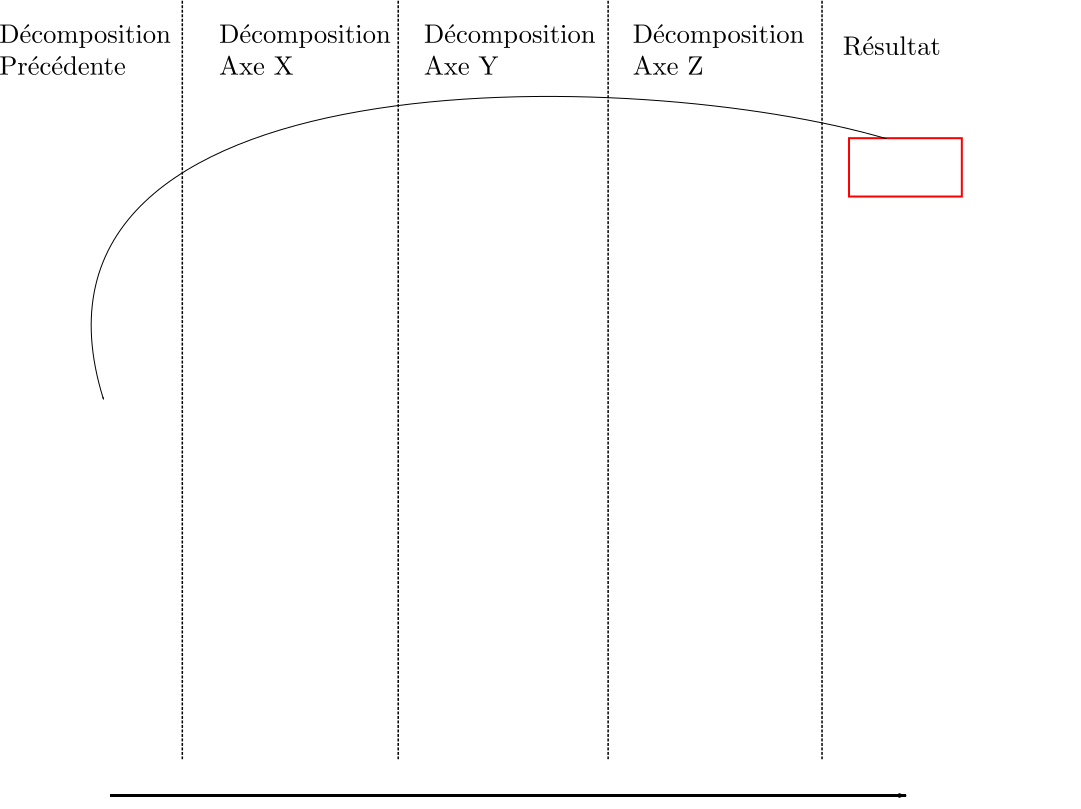
\includegraphics[width=15cm]{images/decompHotell}
 \caption{Décomposition en ondelettes par banc de filtres : Chaque image est filtrée selon les 3 dimensions pour obtenir les coefficients d'ondelettes et d'échelle de chaque voxel de l'image.}
\end{figure}

\subsection{Classifications}

Ce pseudo-code décrit le CAD, de l'importation des images à l'extraction des lésions potentielles:

\begin{enumerate}
 \item Décomposition des images en ondelettes : Pour chaque voxel de l'image d'origine, on obtient entre 8 et 32 coefficients, qui correspondent au vecteur de caractéristiques utilisés par le classifieur
 \item Extraction de la base d'apprentissage : Les coefficients des centres de toutes les tumeurs sont extraits des volumes décomposés, et vont former la base d'apprentissage H1 (lésions). Un certain nombre de voxels sont tirés aléatoirement dans les zones normales de chaque images et leur coefficients sont ajoutés à la base H0 (normale).
 \item Apprentissage : Le classifieur SVM est entraîné sur cette base d'apprentissage pour générer le modèle qui sera utilisé pour le test.
 \item Tests : Le SVM entraîné est utilisé pour classer chaque voxel contenu dans les organes à évaluer (poumon et foie).
 \item Réduction des Faux-positifs : Les points sont agrégés en composantes connexes (connexité 27 en 3 dimensions). Chaque agrégat est testé pour déterminer si il doit être considéré comme un faux positif ou un vrai positif.
\end{enumerate}

\section{Optimisation des paramètres du classifieur}
\label{lab:optim}

Les différentes étapes de l'évaluation des performances nécessitent la fixation d'un grand nombre de paramètres. Tous ceux qui correspondent à l'étape de classification sont adaptés à la modalité à évaluer, tandis que ceux relatifs au processus dans son ensemble sont fixés une seule fois.

\subsection{Paramètres à optimiser pour chaque modalité}

\begin{itemize}
 \item Le terme de pénalisation des exemples mal classés $C$
 \item La largeur de bande $\gamma$ du noyau du classifieur (dans notre cas une RBF - Radial Basis Function, ou fonction de base radiale)
 \item Le niveau de décomposition des images $j$
\end{itemize}

J'ai effectué une recherche exhaustive par grille avec les paramètres suivants :

\begin{description}
 \item [C :] de 1 à 10000 en 15 pas logarithmique
 \item [gamma :] de 0.0001 à 1 en 15 pas logarithmique
 \item [j :] de 1 à 4, soit de 8 à 32 caractéristiques
\end{description}

L'optimisation a été réalisée à l'aide du logiciel rapid-i~\cite{mierswa2006} pour chaque modalité. Les indicateurs de performance (Sensibilité, Spécificité, Précision) sont obtenues en réalisant une validation croisée à 5 étapes sur l'ensemble de la base d'apprentissage. Le triplet de paramètre retenu est celui qui maximise la sensibilité.

Nous avons représenté pour chaque modalité le front de pareto positionnant chaque triplet dans un espace à deux dimensions (`Sensibilité', 'Spécificité'). Cela permet de vérifier que le critère choisit (maximisation de la sensibilité) ne se fait pas trop au détriment de la spécificité.

\subsection{Paramètres globaux}

Trois paramètres sont appliqués sur toutes les données de la même manière :
\begin{description}
 \item[Normalisation :] Les données sont normalisées de manière à ce que la moyenne et l'\emph{écart}-type de chaque caractéristique soit de 1 ($(\mu, \sigma)=(1,1)$) (\emph{moyenne}), ou alors pour que l'ensemble des valeurs soit comprises entre -1 et +1 (\emph{écart}).
 \item[Nombre de points de la base d'apprentissage :] Le nombre de points extraits de chaque image pour alimenter la base d'exemples normaux peut avoir une influence sur les résultats. Trois valeurs sont testées. 100 pts/im. (soit 1500 pts. négatifs), 200 pts/im. (soit 3000 pts. négatifs) et 1000 pts/im. (soit 15000 pts. négatifs).
 \item[positions des points extraits :] Les points normaux extraits de la base d'image peuvent être extraits de tout le volume de l'organe hors tumeurs, ou bien extraits préférentiellement des 
\end{description}

Le but de la normalisation est d'homogénéiser les plages de valeurs des différentes caractéristiques pour faciliter le travail du classifieur, dont les paramètres C et gamma dépendent de la distance entre les points et ne permettent pas de gérer des différences trop importantes d'étendues dans les caractéristiques. La première méthode de normalisation a l'avantage d'être relativement peu sensible aux valeurs extrêmes, contrairement à la seconde.

Le nombre de point de la base d'apprentissage détermine directement la qualité de l'apprentissage. Le nombre de caractéristique est de $8 \times j$, avec $j$ le niveau de décomposition des images. Il n'existe pas de règle définitive pour déterminer le nombre d'exemples nécessaire en fonction du nombre de caractéristiques, mais les SVM sont relativement bon pou éviter le sur-apprentissage. Dans notre cas, il vaudrait donc mieux avoir plus de données. Cependant, le nombre de points notés ``tumeurs'' est limité par le nombre de tumeurs présentes dans la base d'apprentissage (173 tumeurs pour le poumon, 106 pour le foie). Dans ce cas, il y a un risque de déséquilibre de la base d'apprentissage, qui devrait idéalement avoir le même nombre d'exemples ``tumeur'' que ``normales``. Des techniques de correction existent pour les SVM pour contrebalancer ces déséquilibres en indiquant un paramètre C différent pour chaque classe, mais les tests réalisés ne montrent pas d'améliorations significatives des performances.

Les points normaux extraits des images pour alimenter la base vont avoir une influence directe sur la qualité des résultats. Idéalement ils devraient être représentatif de l'ensemble des cas rencontrés dans la base de tests, mais les bordures de certains organes peuvent ressembler à des tumeurs, et rendre l'estimation de la surface de séparation plus difficile. J'ai donc voulu évaluer la performance du CAD sur une base dépourvue des données ambiguës. Pour cela nous avons réalisé une Érosion de 2 voxels sur les le masque des volumes à extraire.

\section{Réduction des faux positifs}

\subsection{Création des agrégats}

Les résultats de la classification des images forment des cartes de score, qui représentent le résultat de la classification pour chaque voxel de l'image source. Ce résultat est donné sous la forme d'un nombre correspondant à la distance entre le vecteur de caractéristique et la surface de séparation. Nous avons choisit une approche par agrégats plutôt que par voxels car elle est plus proche de la réalité de la routine clinique, car le praticien ne travaille pas voxel par voxel mais en indiquant des zones dans l'image.

Les voxels dépassants un seuil prédéterminé sont regroupés selon une connexité 28 ($3\times3\times3$ en 3D). 


\subsection{Critères de sélection des agrégats}

Soit $L$ l'ensemble des points de la lésion, $A$ les points correspondant à l'amas candidat.

Les agrégats seront considérés comme des vrai positifs si ils intersectent une tumeur selon les règles suivantes, comme de faux positifs si ils n'intersectent aucune tumeur. Cependant, si leur taille est inférieure à la taille minimale définie par première règle ($\alpha \times card( L )$), l'amas n'est pas considéré.


\begin{description}
 \item[$card( L \cap A ) > \alpha \times card( L )$] avec $\alpha$ fixé à 0.05 qui fixe la proportion minimale de la tumeur qui doit être présente dans l'amas. Elle permet d'éviter les amas qui intersecteraient la tumeur par accident.
 \item[$card( L \cap A ) > \beta \times card( A )$]  avec $\beta$ fixé à 0.20 limite l'étendue de l'amas en dehors de la tumeur.
\end{description}

\section{Réalisation des courbes Free-ROC}

La réalisation d'une courbe Free-ROC se fait en trois étapes. Tout d'abord, le CAD doit sélectionner un ensemble d'agrégats dans l'image et associer à chacun un score. Ensuite, à partir de la vérité terrain, nous allons déterminer quels agrégats correspondent réellement à une tumeur, ainsi que ceux qui sont de faux positifs. Enfin, la courbe Free-ROC sera tracée en prenant en compte pour chaque niveau de seuil uniquement les agrégats qui sont en dessous de ce seuil.

\subsection{Sélection des clusters candidats}

Les clusters candidats donnés par le CAD sont sélectionnés en binarisant la carte de score pour plusieurs seuils. Le seuil qui permettra d'obtenir la meilleure sensibilité sera sélectionnée.

Cette sélection est réalisée selon l'algorithme suivant :

\begin{itemize}
 \item \emph{Sensibilité} := Dictionnaire vide
 \item Pour chaque seuil \emph{s} entre -2 et +2 (40 pas), faire :
 \item \hspace{1cm}\emph{CarteSeuillée} := Seuiller \emph{carte de Score} au seuil \emph{s}
 \item \hspace{1cm}\emph{Agrégats} := Calcul des agrégats de \emph{CarteSeuillée} (Score, classe, étendue).
 \item \hspace{1cm}Sensibilité[s] := Calcul Sensibilité(Agrégats)
 \item fin faire
 \item \emph{Seuil Optimal} := Seuil qui maximise la Sensibilité
\end{itemize}

Ce critère de sélection va naturellement engendrer un grand nombre de faux positifs, mais il faut garder à l'esprit qu'il sera utilisé pour réaliser des courbes F-ROC, qui indiquent une spécificité pour chaque nombre de faux positif en jouant sur le seuil.

\chapter{Analyse des résultats}

Dans ce chapitre je vais détailler les résultats obtenus par les méthodes présentées précédemment. Je commencerais par présenter les courbes obtenues lors de l'étape d'optimisation et d'adaptation du CAD aux données, puis je parlerais des résultats obtenus par ce CAD pour les différentes modalités.

\section{Optimisation des paramètres}


\begin{figure}[h!]
\label{fig:paretoParams1}
\begin{center}
 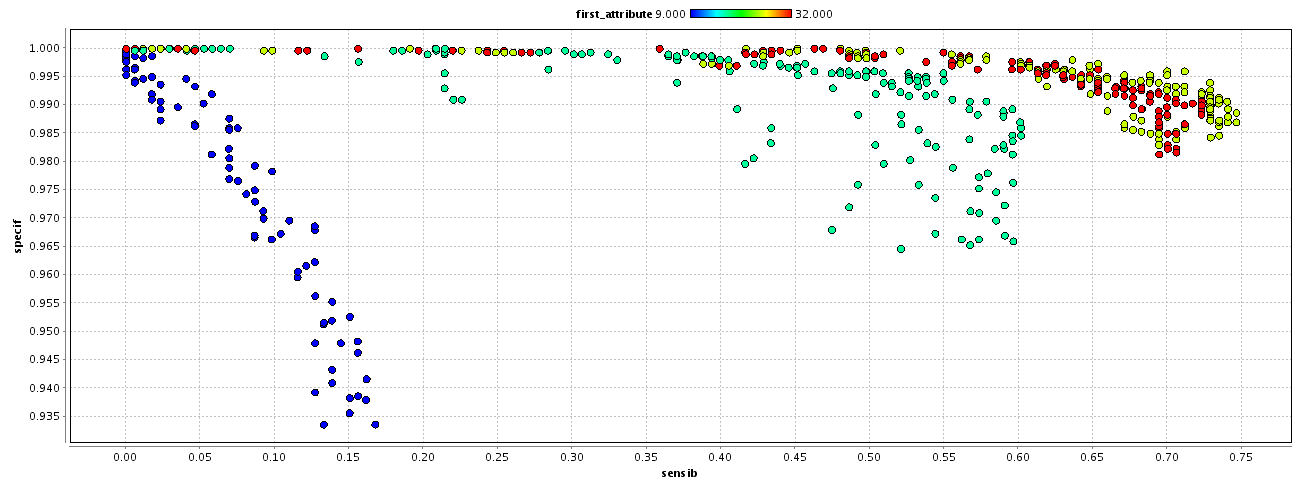
\includegraphics[width=14cm]{images/pareto_param_200.png}

{\small a) Base Témoin}
\vspace{0.5cm}

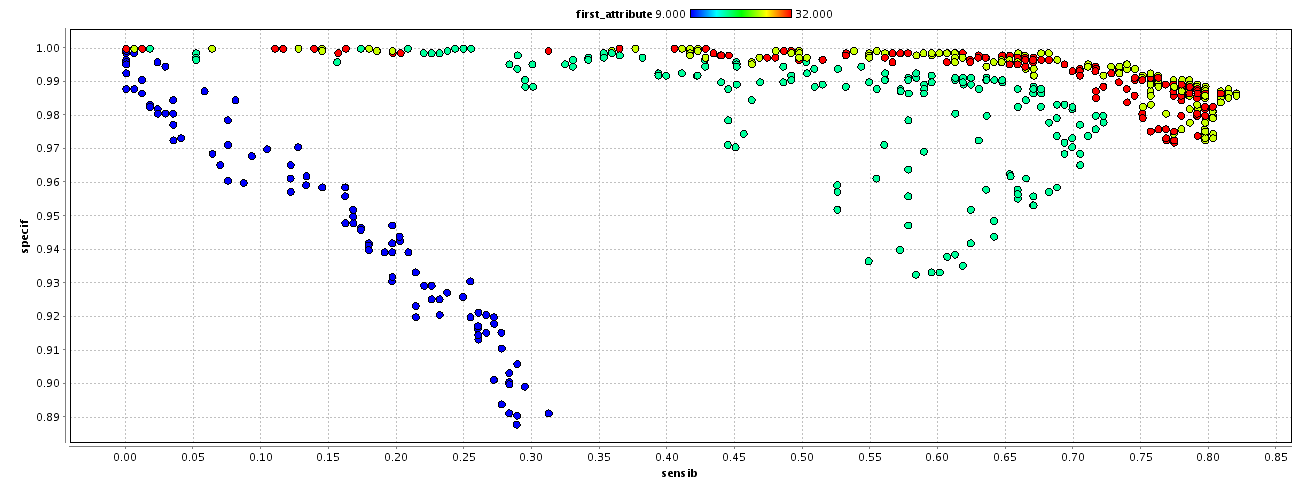
\includegraphics[width=14cm]{images/pareto_param_100.png}

{\small b) Base appauvrie}


 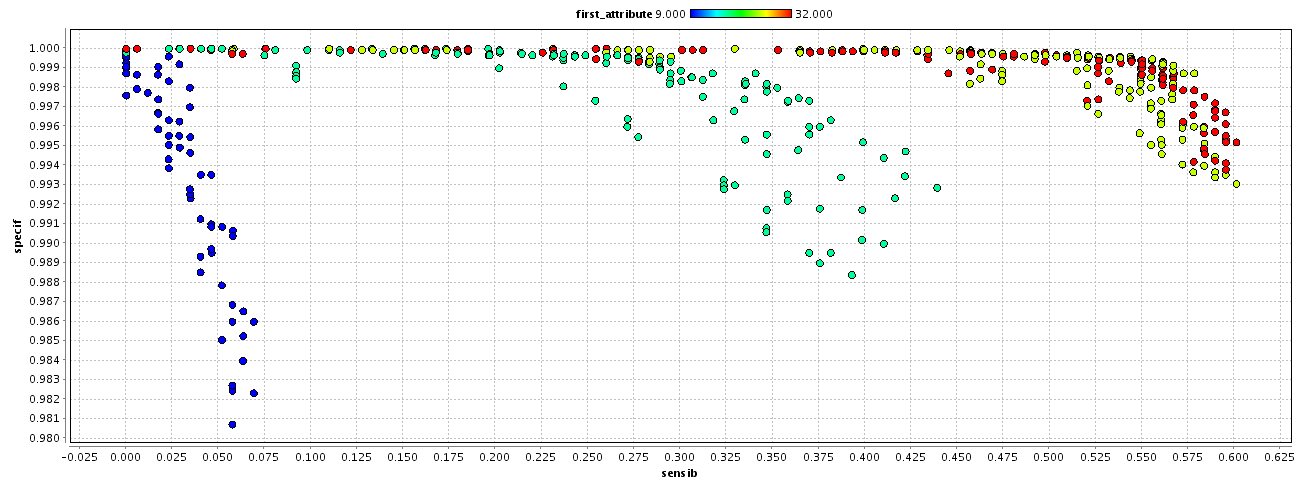
\includegraphics[width=14cm]{images/pareto_param_1000.png}
 
{\small c) Base enrichie}



\end{center}
 \caption{Fronts de pareto des résultats de la recherche des meilleurs paramètres du classifieur (1/2). Pour chaque triplet de paramètres (C, $\gamma$, j), la sensibilité et la spécificité sont reportées sur le graphique. Le code couleur correspond à la valeur de j. En a), la base témoin, avec 200 points négatifs par image et une normalisation \emph{moyenne}, en b) la base appauvrie avec 100 points négatifs par image et une normalisation \emph{moyenne}, et en c) la base enrichie avec 1000 points négatifs par image et une normalisation \emph{moyenne}.}
\end{figure}



\begin{figure}[h!]
\label{fig:paretoParams2}
\begin{center}

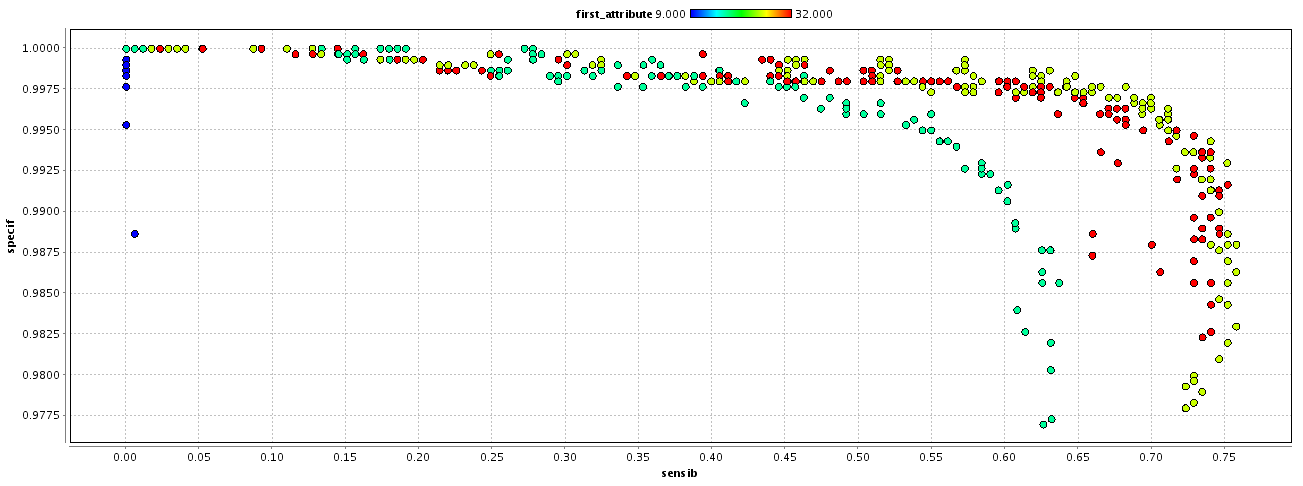
\includegraphics[width=14cm]{images/pareto_param_range.png}

{\small d) Base Normalisée -1/+1}

\vspace{0.5cm}

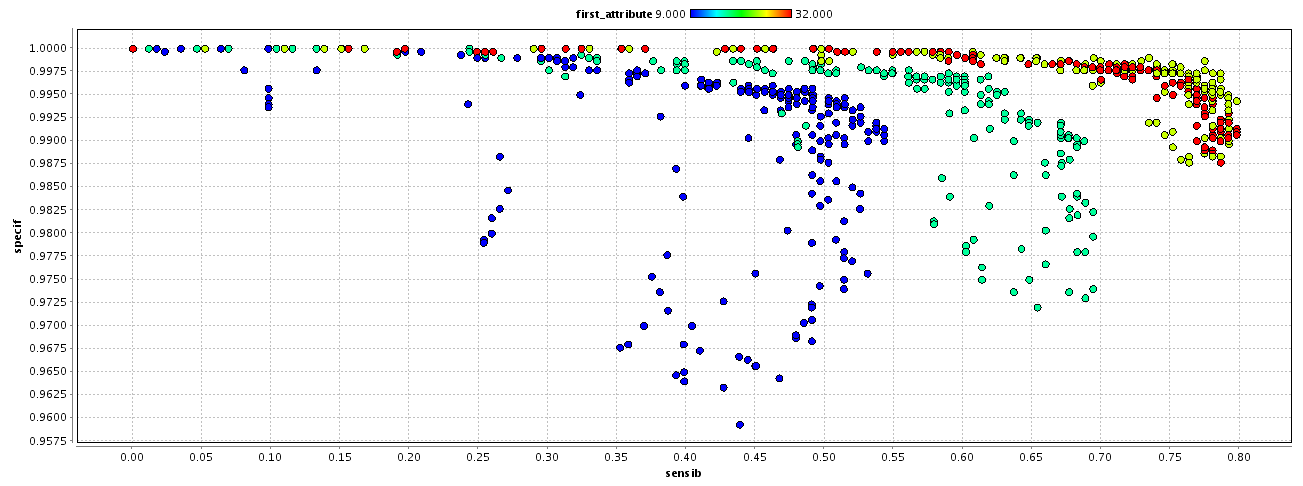
\includegraphics[width=14cm]{images/pareto_param_erosion.png}

{\small d) Base \'Erodée}


\end{center}
 \caption{Fronts de pareto des résultats de la recherche des meilleurs paramètres du classifieur (2/2). Pour chaque triplet de paramètres (C, $\gamma$, j), la sensibilité et la spécificité sont reportées sur le graphique. Le code couleur correspond à la valeur de j. En a) la base normalisation avec 200 points négatifs par image et une normalisation +1/-1. En b), la base érodée, avec 200 points négatifs par image et une normalisation \emph{moyenne}, en b) la base enrichie avec 1000 points négatifs par image et une normalisation \emph{moyenne}. }
\end{figure}




\begin{figure}[h!]
\label{fig:paramsParams}
%	\begin{center}
		\begin{tabular}{c c c c c c}
  \hline
  a	& Base Témoin 	& Base Érosion	& Base appauvrie& Base enrichie & Base normalisée \\
  \hline
 C 	& 464		& 74		& 5412		& 5412		& 10000 \\
\hline
$\gamma$& 0.0053	& 0.0094	& 0.00031	& 0.0017	& 0.052 \\
\hline
j	& 3		& 3		& 3		& 4		& 3	\\
\hline
\hline
Sensibilité& 0.75	& 0.80		& \textbf{0.82}		& 0.60		& 0.76	\\
\hline
Spécificité& 0.99	& 0.99		& 0.99		& 0.99		& 0.99 \\
\hline
Précision& 0.98		& 0.98		& 0.97		& 0.99		& 0.98 \\
\hline
 		\end{tabular}

%	\end{center}
\caption{Paramètres sélectionnés pour l'optimisation des performances. Sont indiqués pour chaque base le triplet de paramètres sélectionné ainsi que sa position sur le front de pareto.}
\end{figure}






Nous avons réalisé des mesures de performances pour 5 jeux de paramètres différents présentés ci-après. Les paramètres en \emph{gras} correspondent à ceux utilisés pour la base témoin.

\begin{itemize}
 \item Nombre de points de la base d'apprentissage (100, \emph{200}, 1000)
 \item Normalisation des données (\emph{moyenne}, +1/-1)
 \item Position des points de la base d'apprentissage (\emph{organe}, Érosion)
\end{itemize}


\begin{description}
 \item[Témoin : ] contient des données normalisées par la méthode moyenne avec 200 points extraits de chaque organe.
 \item[\'Erosion : ] contient des données normalisées par la méthode moyenne avec 200 points extraits de chaque organe érodée.
 \item[Appauvrie : ] contient des données normalisées par la méthode moyenne avec 100 points extraits de chaque organe.
 \item[Enrichie : ] contient des données normalisées par la méthode moyenne avec 1000 points extraits de chaque organe.
 \item[Normalisation : ] contient des données normalisées par la méthode +1/1 avec 200 points extraits de chaque organe.
\end{description}


\subsubsection{Sélection des meilleurs paramètres du classifieur}

Les paramètres du classifieur sont déterminés par une recherche par grille. Elle consiste à rechercher l'optimum en évaluant la performance ce chaque jeu de paramètre dans un ensemble déterminé à l'avance pour représenter . La performance de chaque triplet (C, $\gamma$, j) est estimée en réalisant une cross-validation à 5 validations sur l'ensemble de la base d'apprentissage.

Les performances de tous les jeux de paramètres sont représentés sous la forme d'un front de pareto. Ce type de diagramme permet de rechercher un optimum selon plusieurs critères incompatibles. Dans notre cas, nous voulons à la fois une sensibilité et une spécificité importante, sachant qu'il n'existe pas de jeu de paramètres ''parfaits`` qui permettent d'avoir 100\% aux deux. Dans notre cas, le front de pareto va permettre de vérifier que le choix par maximisation de la sensibilité ne se fait pas au détriment de la spécificité.

Les paramètres sont choisis à partir du front de pareto figure \ref{fig:paretoParams1} en maximisant la sensibilité.

Dans l'ensemble, on peut voir clairement que les points correspondant au premier niveau de décomposition (bleu foncé) ont une performance systématiquement inférieure aux autres. Pour la base témoin, la performance maximal est atteinte pour environ 15\% de sensibilité et une spécificité de 93.5\%, ce qui correspond à la valeur de spécificité la plus faible de tous les points de la base témoin. On observe cependant un front de pareto marqué, bien qu'en fort retrait par rapport aux autres niveaux de décomposition. Ce même constat se retrouve pour les bases appauvries et enrichies.

Les deux autres bases ont des comportements différents. Pour la base normalisée, les performances s'effondrent suffisamment pour que le classifieur soit quasiment incapable de discerner les classes, avec une sensibilité maximale de 1\% environ. Cela indique qu'il ne parvient pas à trouver une surface de séparation des données avec les paramètres indiqués. Puisque la normalisation moyenne parvient à mieux séparer les données pour ce niveau de décomposition, il est probable que la normalisation ne parvienne pas à homogénéiser les différentes dimensions de manière satisfaisante. Dans le cas de la base érodée, la simplification du problème de classification fait que les performances sont nettement en hausse avec des performances de l'ordre de 55\% de sensibilité pour 99.2\% de spécificité, ce qui est le score le plus élevé de toutes les bases.

Les performances du second niveau de décomposition (bleu ciel) sont toujours situées environ au barycentre entre les performances du premier niveau et celles des niveaux 3 et 4.

Les performances des décomposition de niveaux 3 (vert) et 4 (rouge) sont systématiquement meilleures que les autres mais sont entremêlées. La base Témoin et la base Appauvrie montrent une claire avance tant en terme de sensibilité que de spécificité pour 3 niveaux de décomposition. La base érodée ne montre quand à elle aucune différence de spécificité entre ces deux niveaux de décomposition, mais montre cependant une faible amélioration de la sensibilité pour les 4 niveaux (de 0.5\%). Quand à la base normalisée, on n'observe pas de réelles différences entre les deux niveaux de décomposition.

La figure \ref{fig:paramsParams} référence tous les paramètres sélectionnés à partir des courbes de pareto. On peut observer que la sensibilité la plus importante est atteinte pour la base appauvrie, avec 82\% de bonne détection. Ce taux est sensiblement le même que celui de la base Érosion (80\%). Ces valeurs importantes par rapport aux autres peuvent s'expliquer par le fait que ces deux bases proposent un problème simplifié. Dans le cas de la base Érosion, les cas litigieux (discontinuités proches des bords des organes) ont été retirés de la base, ce qui simplifie le problème, tandis que pour la base appauvrie, c'est le nombre de points ''sain`` plus faible de la base d'apprentissage (1500 contre 3000) qui permet de rendre le problème plus simple à traiter au détriment de la généralisation du résultat trouvé aux images complètes.

Il est intéressant de constater que les performances en sensibilité pour les bases Appauvrie, Témoin et Enrichie sont inversement proportionnels à la taille de la base. En effet, plus la complexité de la base est importante, plus il devient difficile de trouver une surface de séparation efficace. Cependant, une base trop simpliste va engendrer une solution qui sera sans rapport avec la réalité, comme nous le verrons plus tard avec les courbes F-ROC.

Les valeurs de spécificité sont toutes très supérieures à 99\%, ce qui montre que le classifieur n'a pas de problèmes pour classer correctement les points sains. En effet, la base étant très déséquilibrée, avec un rapport de 17 points sains pour 1 point ''lésion`` dans la base témoin, il est normal il est normal que le classifieur favorise la classification des points ''sain''. Il existe des techniques permettant de compenser ce déséquilibre lors de l'apprentissage, mais tous les tests que nous avons réalisés n'ont pas montrés d'amélioration du résultat. En effet, l'étape de sélection du seuil (voir section suivante) permet de compenser ces différences.

\subsection{Courbe Free-ROC}

Les courbes Free-ROC de la figure \ref{lab:froc_comp_static} permettent de comparer les performances du CAD sur les différentes bases d'apprentissage. Les courbes ont volontairement été tronquées à 40 faux positifs par image, car ce nombre est déjà trop important pour un système CAD.

On peut observer que les courbes correspondants aux bases Témoin et Enrichie atteignent leur maximum de performances pour un nombre de faux positifs relativement faible par rapport aux autres bases : entre 17 et 20 faux positifs pour ces bases, contre plus de 40 pour les bases Appauvrie et \'Erosion. Cela tends à montrer que le système CAD est plus performant pour ces bases car il crée moins d'agrégats là ou il n'y a pas de lésions.

En ce qui concerne la sensibilité maximale obtenue sur les courbes, elle est atteinte pour la base témoin avec environ 62\% de sensibilité, suivie par la base appauvrie avec 60\%, mais pour un nombre de faux positifs beaucoup plus important (38 contre 18 pour la base Témoin). La troisième courbe est la courbe Normalisation, suivie par la base enrichie puis la base \'Erosion. Il est important de noter que les sensibilités maximales observées sont très proches, entre 55\% et 62\%, ce qui indique que la qualité de la base d'apprentissage n'a pas d'impact réel sur la sensibilité maximale atteinte par le CAD, mais qu'il pourra être plus ou moins difficile pour ce dernier de différencier les lésions du bruit de fond. 

En pratique, on choisira le seuil pour avoir la certitude d'avoir un nombre de faux positifs ``raisonnable'' par image. Dans notre cas, les images contiennent environ 10 lésions par image. Il peut être intéressant de comparer les performances des bases pour ratio de 1 faux positif par lésion, soit pour 10 faux positifs. Dans ce cas, la base Témoin est au coude à coude avec la base Enrichie, à environ 55\%, ce qui est déjà très proche de leur performances maximales. La base Normalisation et la base Appauvrie sont quand à elles à 40\% de sensibilité, tandis que la base Érosion atteint 35\%.

Dans tous les cas, nous avons donc vu que le maximum de performances est apporté par la base Témoin.

\begin{figure}[h!]
 
 \begin{center}
   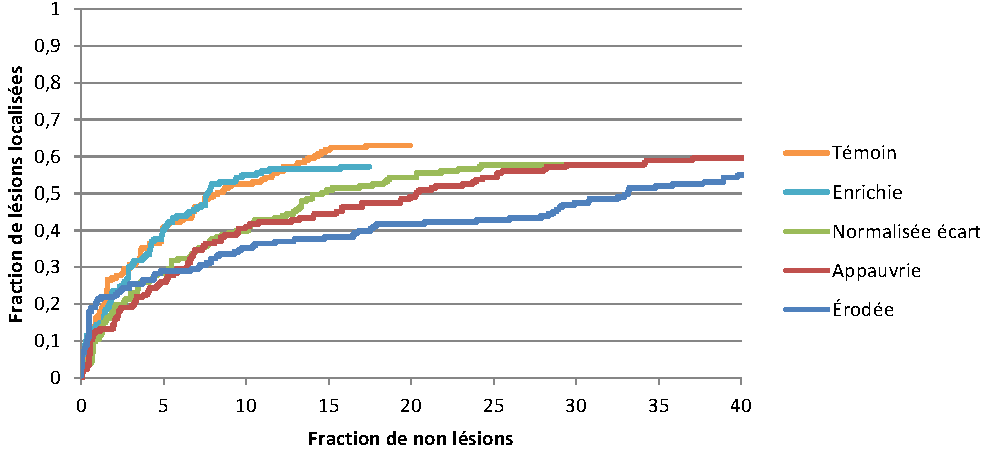
\includegraphics[width=15cm]{images/FROC_param}
 \end{center}
 \label{lab:froc_comp_static}
 \caption{Courbe Free-ROC comparant les performances du CAD sur une base témoin (normalisation \emph{moyenne} et 200 points négatifs par image), sur une base enrichie (1000 points négatifs par image), sur une base appauvrie (100 points négatifs par image), sur une base normalisée différemment (normalisation entre -1 et +1 et 200 points négatifs par image) et enfin sur une base de 100 points négatifs par image mais dont les volumes ont été érodés de 2 voxels.}

\end{figure}


\subsection{Comparaison des performances JAFROC}

La comparaison des performances obtenues par l'algorithme JAFROC\cite{chakraborty1990free} nous montre les FDM (Figure de Mérite) obtenues pour les différentes bases. La FDM des bases Témoin, Érosion et Enrichie sont quasiment au même niveau à 0.18, mais les barres d'erreurs semblent montrer un léger avantage pour la base Témoin\ref{lab:fom_param}.

Les bases Normalisation et Appauvrie quand à elles ont une FDM de 0.1 environ, ce qui indique une performance plus faible que les autres.

D'un point de vue statistique, La p-value fournie par le logiciel est de 0.049, ce qui ne permet pas de pouvoir annoncer avec une fiabilité de 95\% que le test est significatif, c-à-d que les FDM sont effectivement toutes différentes. Cela se vérifie aisément en regardant l'étendue des barres d'erreur. Mais il faut noter que cette FDM est basée sur une méthode avec une puissance statistique faible, ce qui signifie qu'elle sous-estime la p-value.


\begin{figure}[h!]
 \begin{center}
   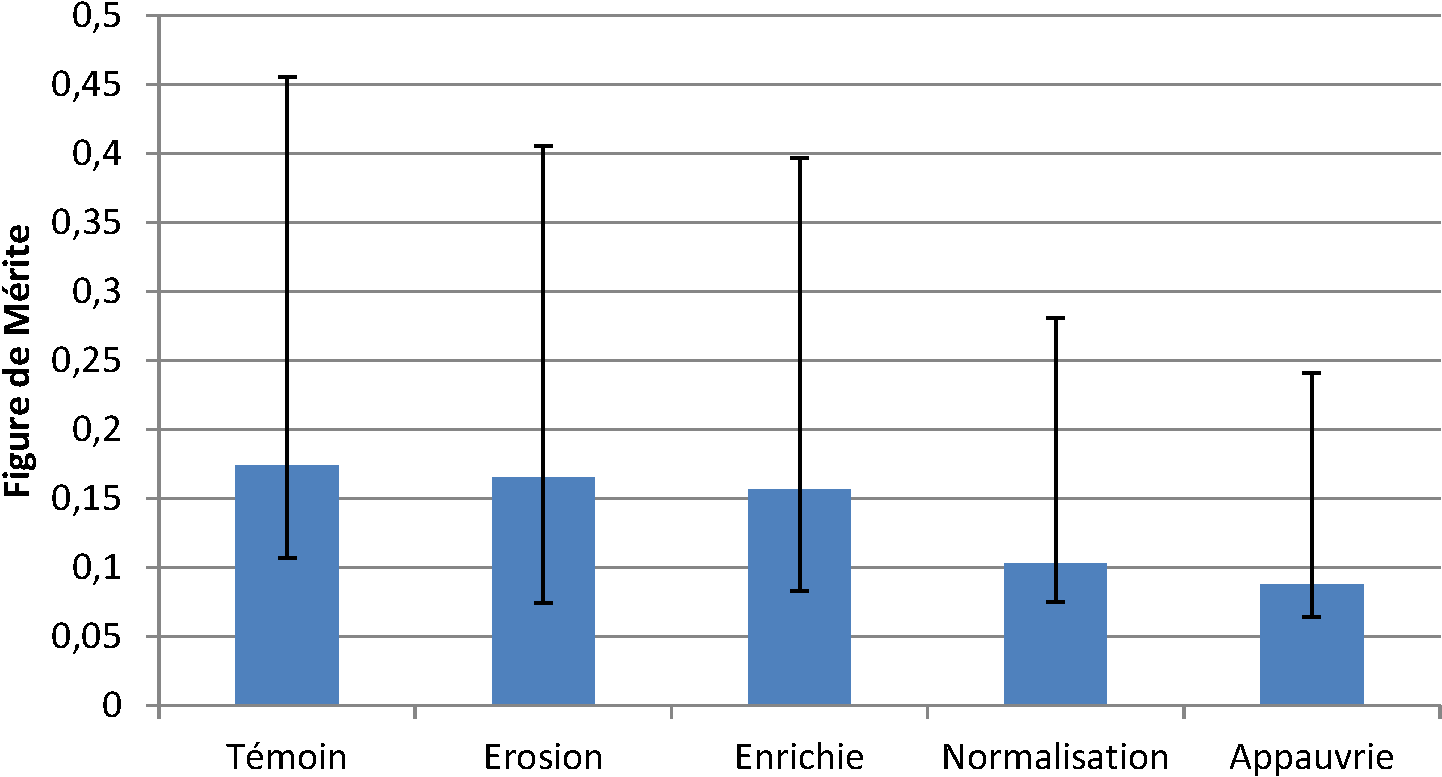
\includegraphics[width=15cm]{images/FOM_param}
 \end{center}
 \caption{ \label{lab:fom_param} Les FOM (Figure de Mérite) obtenues pour les différents paramètres}
\end{figure}

\FloatBarrier

\section{Comparaison des performances des différentes méthodes Poumon}

Les caractéristiques utilisées pour obtenir ces résultats sont les suivants :

\begin{itemize}
 \item 200 points tirés aléatoirement dans le volume de chaque image (hors tumeurs)
 \item normalisation par moyennage et neutralisation de la variance 
\end{itemize}


\begin{figure}[h!]

\begin{center}
 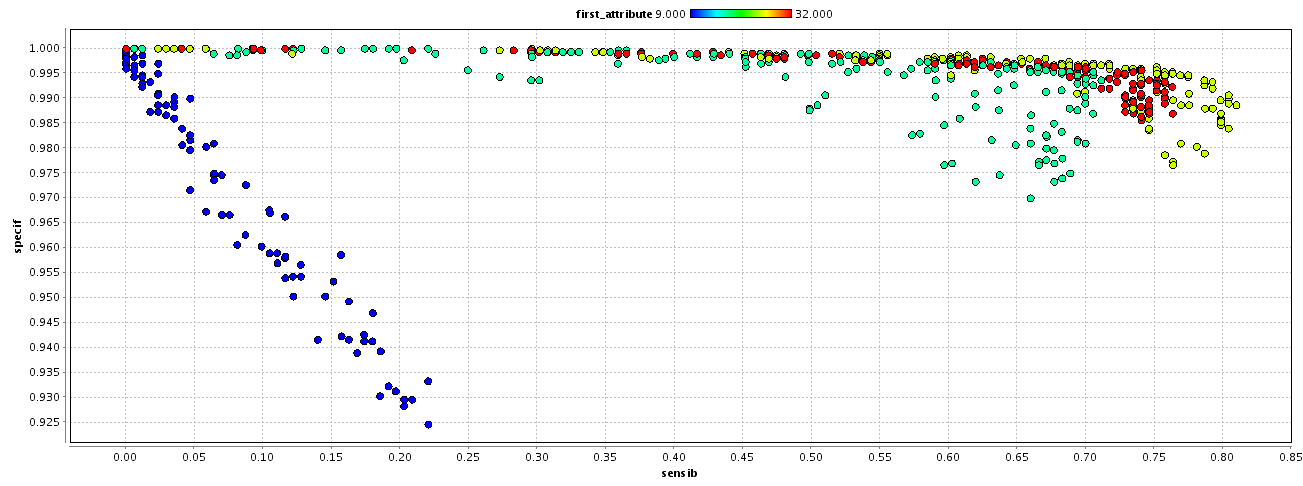
\includegraphics[width=14cm]{images/pareto_mod_IM.png}

{\small a) ET-IM}
\vspace{0.5cm}

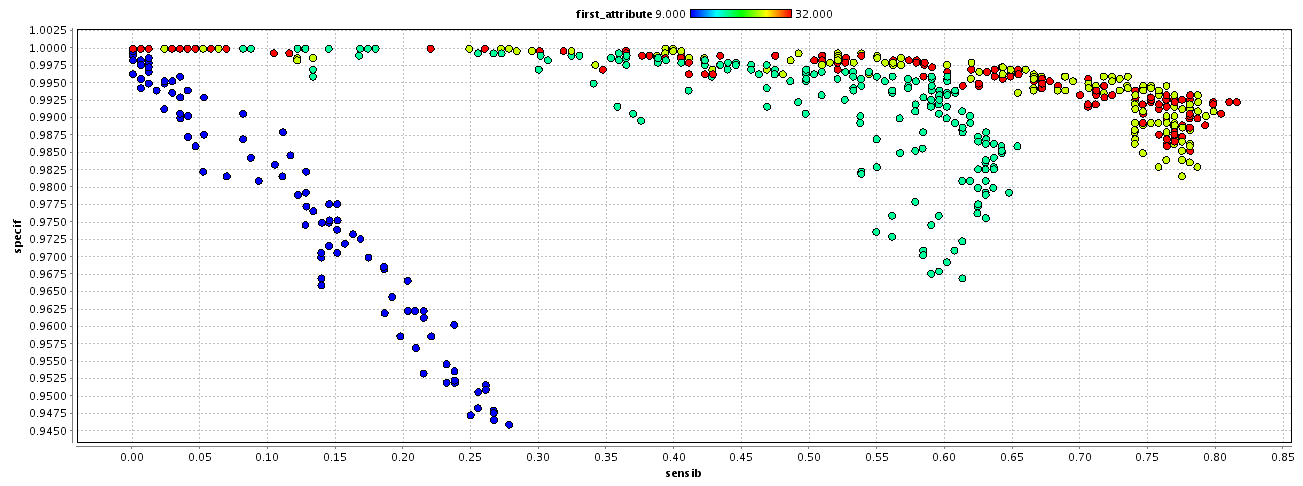
\includegraphics[width=14cm]{images/pareto_mod_LOR.png}
 
{\small b) ET-LOR}
\vspace{0.5cm}

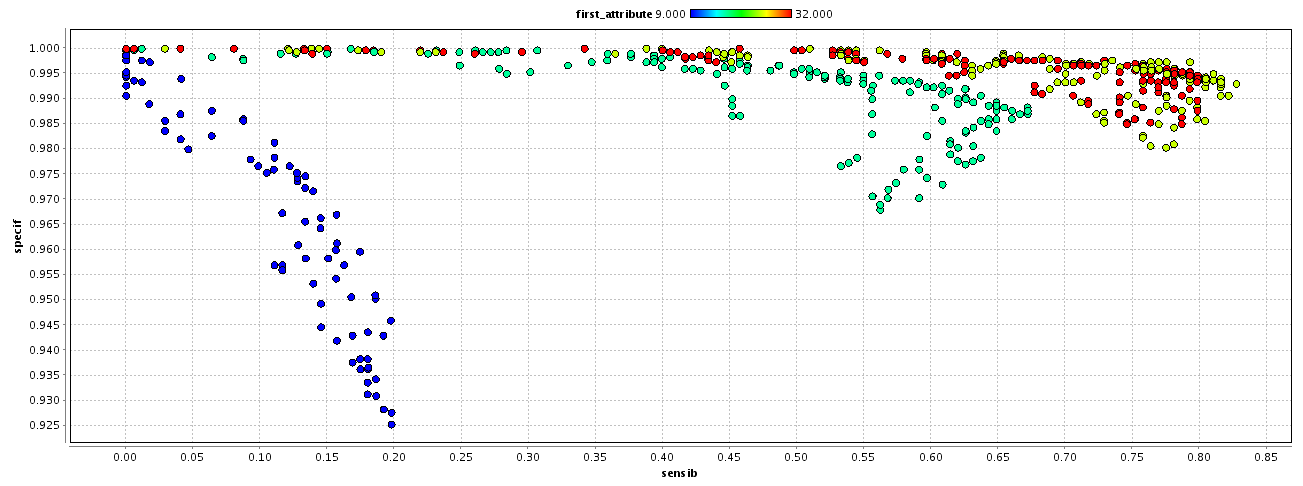
\includegraphics[width=14cm]{images/pareto_mod_NoCorr.png}

{\small c) ET-NoCorr}

\end{center}
 \caption{\label{fig:paretoModalite} Fronts de pareto des résultats de la recherche des meilleurs paramètres du classifieur pour les différentes modalités, avec 200 points négatifs par image. Pour chaque triplet de paramètres (C, $\gamma$, j), la sensibilité et la spécificité sont reportées sur le graphique. Le code couleur correspond à la valeur de j. a) représente la correction d'image ET-IM, b) les images non corrigées du mouvement, et c) les images corrigées par la méthode LOR.}
\end{figure}








\begin{figure}[h!]
\label{fig:paramsModPoumon}
%	\begin{center}
		\begin{tabular}{c| c c c c c}
  \hline
  a	& Base Statique	& Base IM	& Base LOR	& Base NoCorr	\\
  \hline
 C 	& 464		& 10000		& 10000		& 10000		\\
\hline
$\gamma$& 0.0053	& 0.00097	& 0.00031	& 0.00055	\\
\hline
j	& 3		& 3		& 4		& 3		\\
\hline
\hline
Sensibilité& 0.75	& 0.81		& 0.82		& 0.83	\\
\hline
Spécificité& 0.99	& 0.99		& 0.99		& 0.99		\\
\hline
Précision& 0.98		& 0.98		& 0.98		& 0.98		\\
\hline
 		\end{tabular}

%	\end{center}
\caption{Paramètres sélectionnés pour l'optimisation des performances du Poumon. Sont indiqués pour chaque base le triplet de paramètres sélectionné ainsi que sa position sur le front de pareto.}
\end{figure}



\emph{ET-IM}

Cette base contient des données normalisées par la méthode mean/std. avec 200 points extraits de chaque image.




\emph{ET-LOR}

Cette base contient des données normalisées par la méthode mean/std. avec 200 points extraits de chaque image.


\emph{ET-NoCorr}

Cette base contient des données normalisées par la méthode mean/std. avec 200 points extraits de chaque image.


\subsection{Comparaison des performances JAFROC}

La p-value est de 0.10, ce qui ne permet pas de déclarer que statistiquement les données sont différentes : \ref{lab:fom_mod19}.

\begin{figure}[h!]
 \begin{center}
   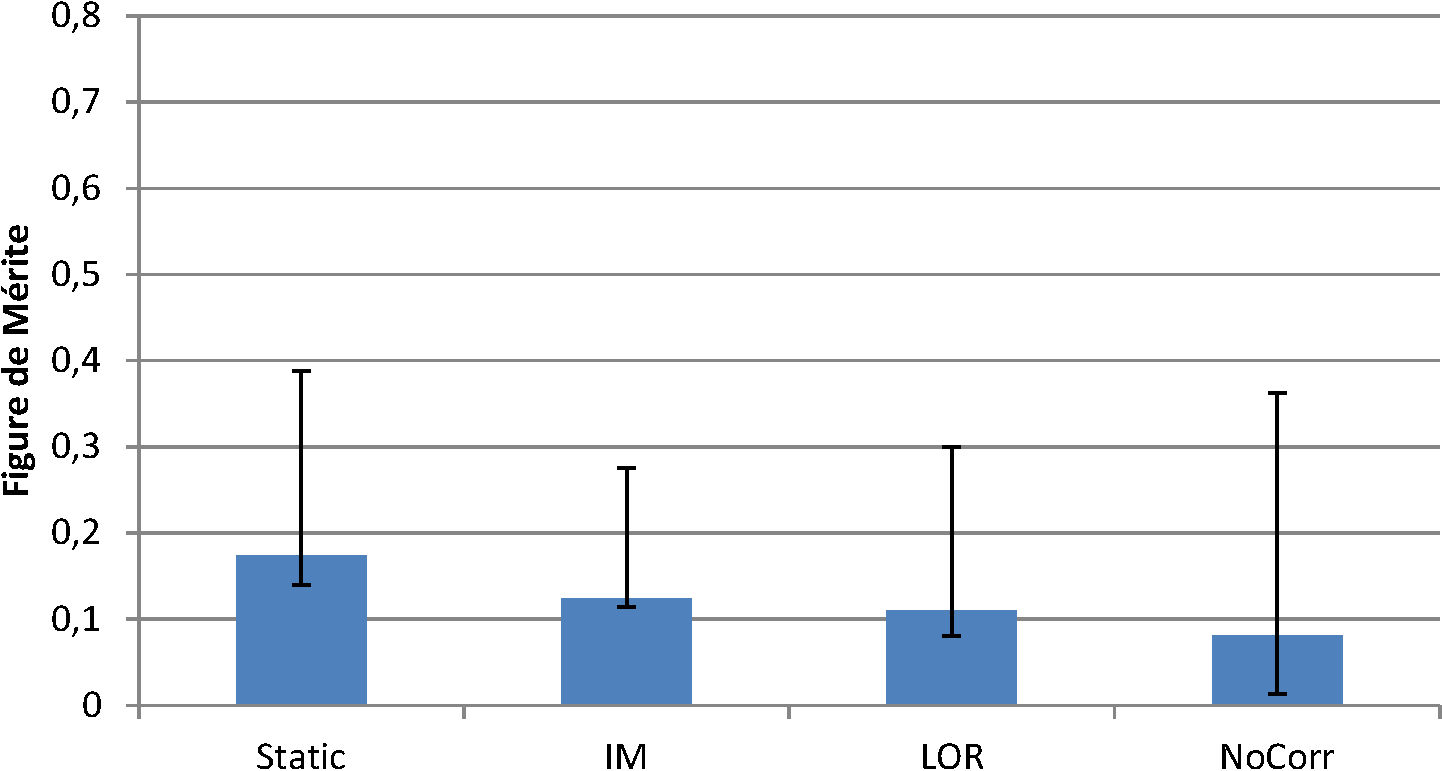
\includegraphics[width=15cm]{images/FOM_mod}
 \end{center}
 \caption{ \label{lab:fom_mod19} Les FDM (Figure de Mérite) obtenues pour les différentes modalités.}
\end{figure}

\subsection{Courbes Free-ROC}

Voir figure \ref{lab:froc_mod}.
Le maximum de performances est apporté par les images statiques, suivi par les images ET-IM.

\begin{figure}[h!]
 \begin{center}
   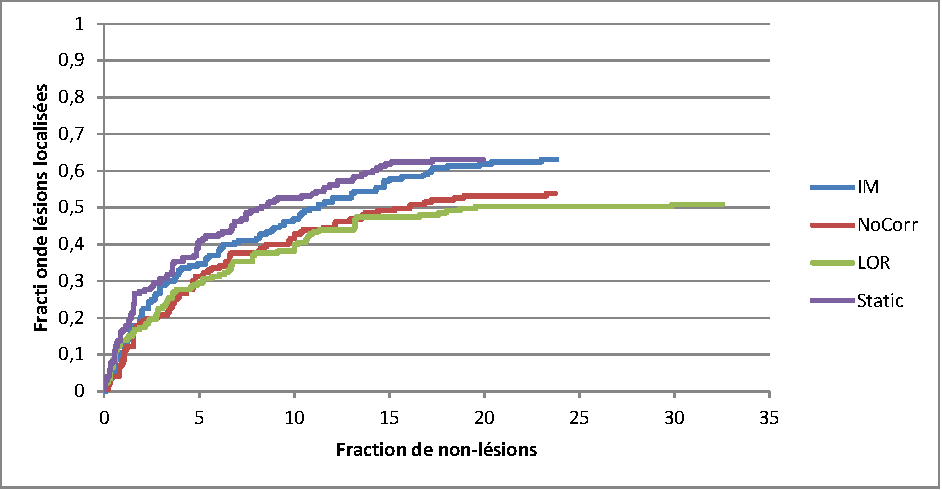
\includegraphics[width=15cm]{images/FROC_mod}
 \end{center}
 \caption{ \label{lab:froc_mod} Courbe Free-ROC comparant les performances du CAD selon les modalités de correction du mouvement respiratoire.}
\end{figure}


\FloatBarrier

\section{Comparaison des performances des différentes méthodes Foie}

Les caractéristiques utilisées pour obtenir ces résultats sont les suivants :

\begin{itemize}
 \item 200 points tirés aléatoirement dans le volume de chaque image (hors tumeurs)
 \item normalisation par moyennage et neutralisation de la variance 
\end{itemize}

\subsection{Comparaison des performances JAFROC}

La p-value est de 0.1, ce qui ne permet pas de déclarer que statistiquement les données sont différentes : \ref{lab:fom_mod19}


\begin{figure}[h!]
 \begin{center}
   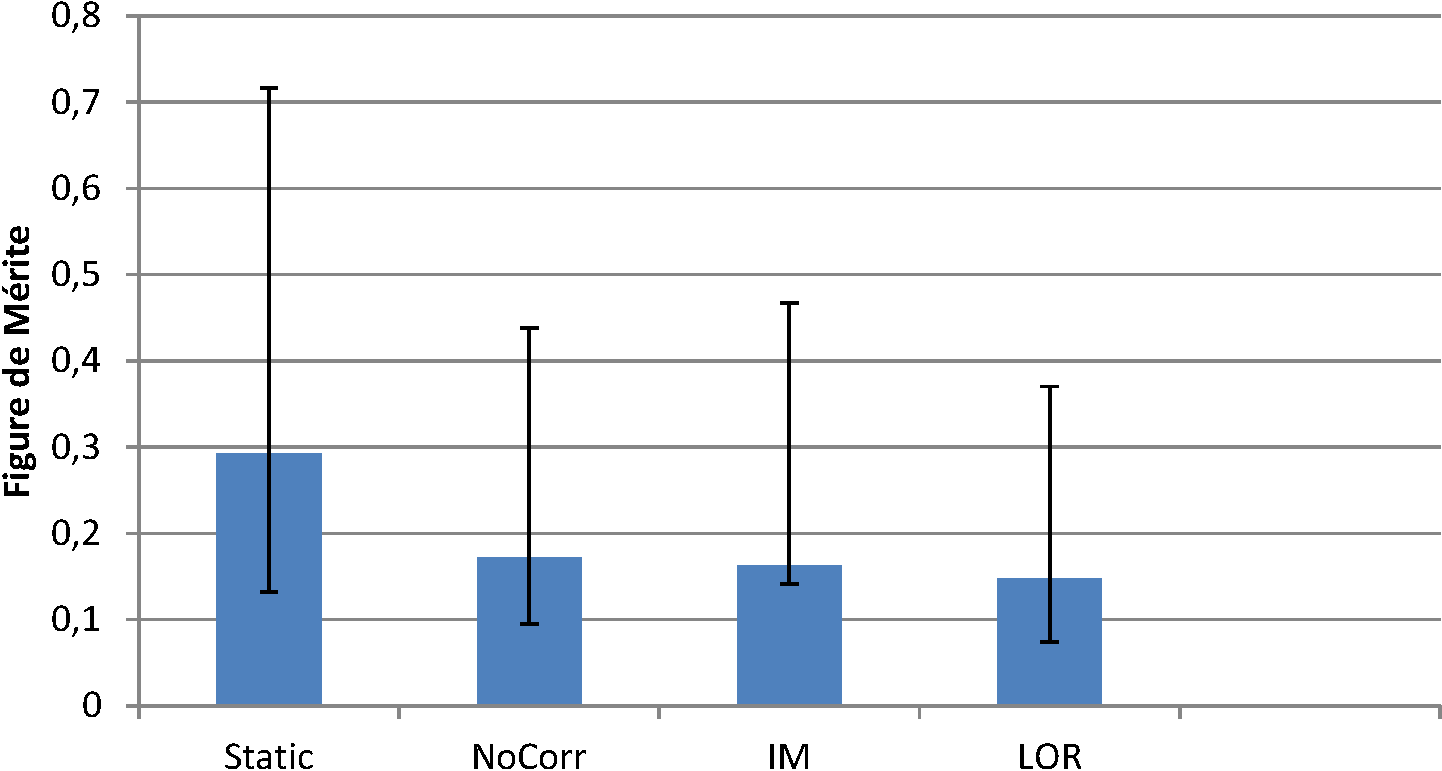
\includegraphics[width=15cm]{images/FOM_mod19}
 \end{center}
 \caption{ \label{lab:fom_mod19} Les FDM (Figure de Mérite) obtenues pour les différentes modalités.}
\end{figure}


\subsection{Courbes Free-ROC}

Voir figure \ref{lab:froc_mod19}.
Le maximum de performances est apporté par les images statiques, suivi par les images ET-IM.

\begin{figure}[h!]
 \begin{center}
   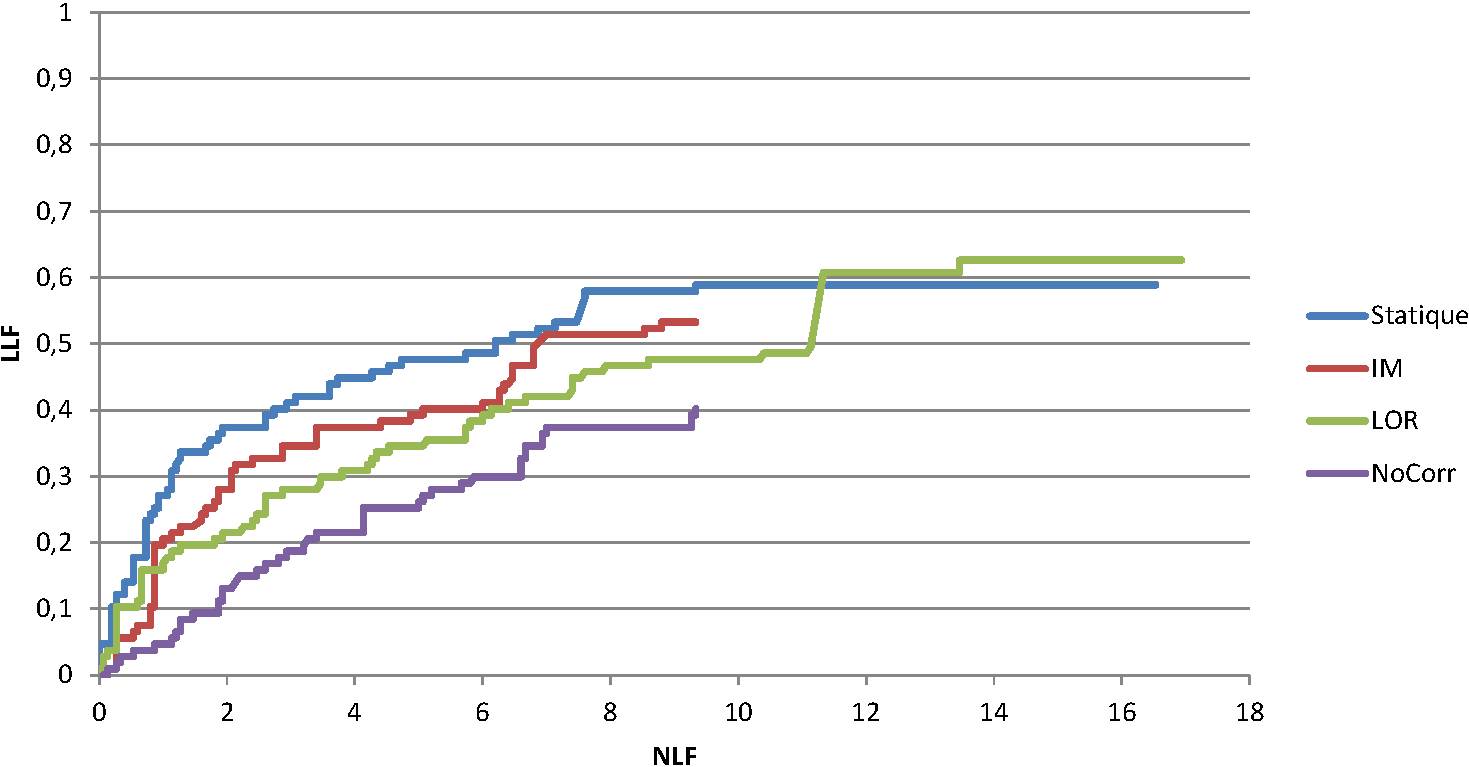
\includegraphics[width=15cm]{images/FROC_mod19}
 \end{center}
 \caption{ \label{lab:froc_mod19} Courbe Free-ROC comparant les performances du CAD selon les modalités de correction du mouvement respiratoire.}
\end{figure}


\begin{figure}[h!]

\begin{center}
 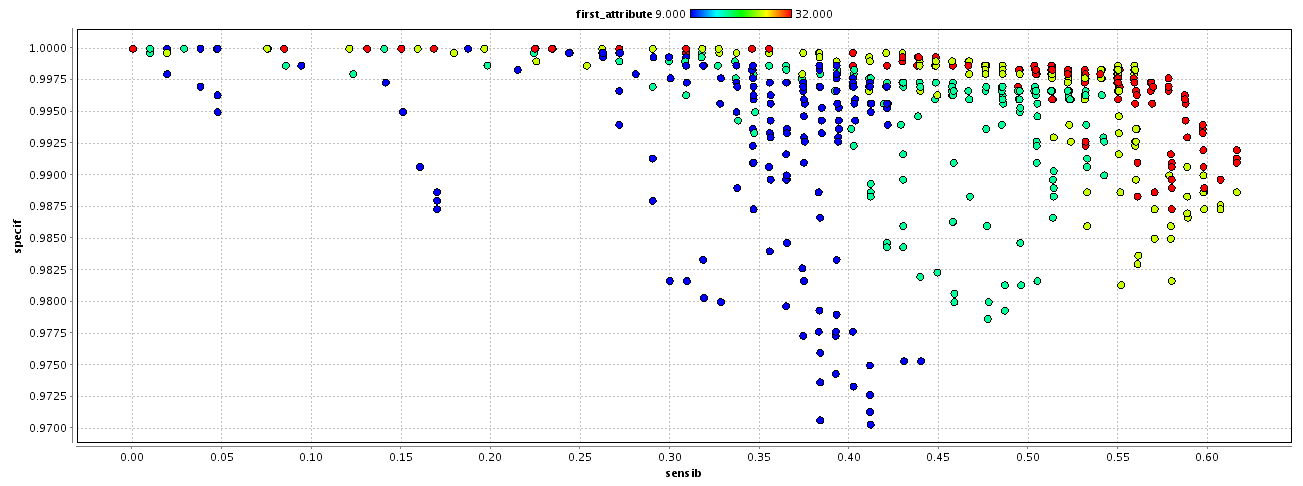
\includegraphics[width=14cm]{images/pareto_mod_Static19.png}

{\small a) ET-Static}
\vspace{0.5cm}

 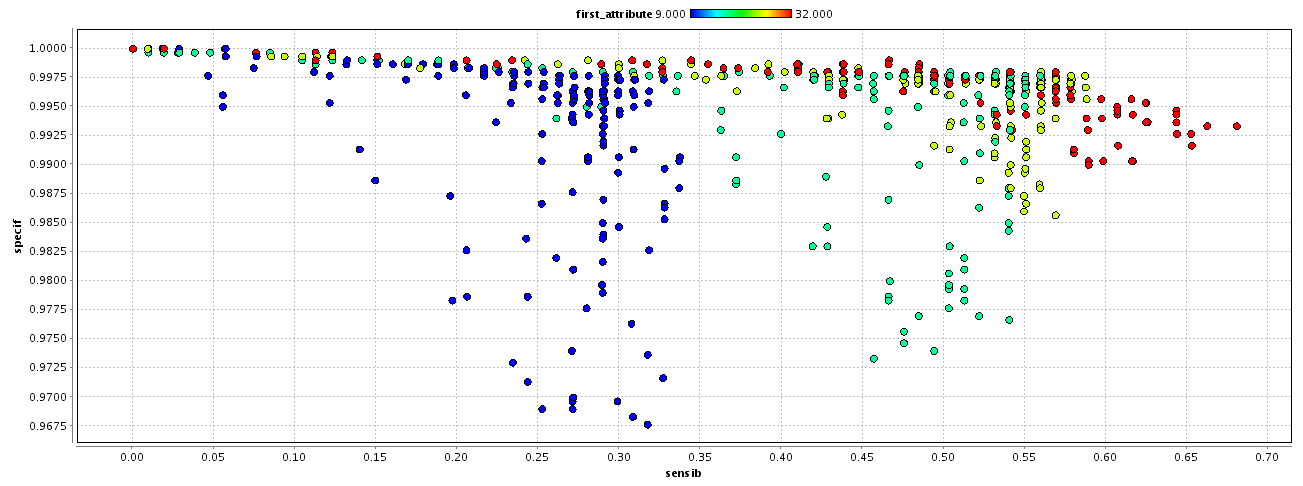
\includegraphics[width=14cm]{images/pareto_mod_IM19.png}

{\small b) ET-IM}

\end{center}
 \caption{\label{fig:paretoModalite19_1} Fronts de pareto des résultats de la recherche des meilleurs paramètres du classifieur pour les différentes modalités, avec 200 points négatifs par image. Pour chaque triplet de paramètres (C, $\gamma$, j), la sensibilité et la spécificité sont reportées sur le graphique. Le code couleur correspond à la valeur de j. a) représente la correction d'image ET-Static, b) les images corrigées du mouvement post-reconstruction.}
\end{figure}

\begin{figure}[h!]

\begin{center}
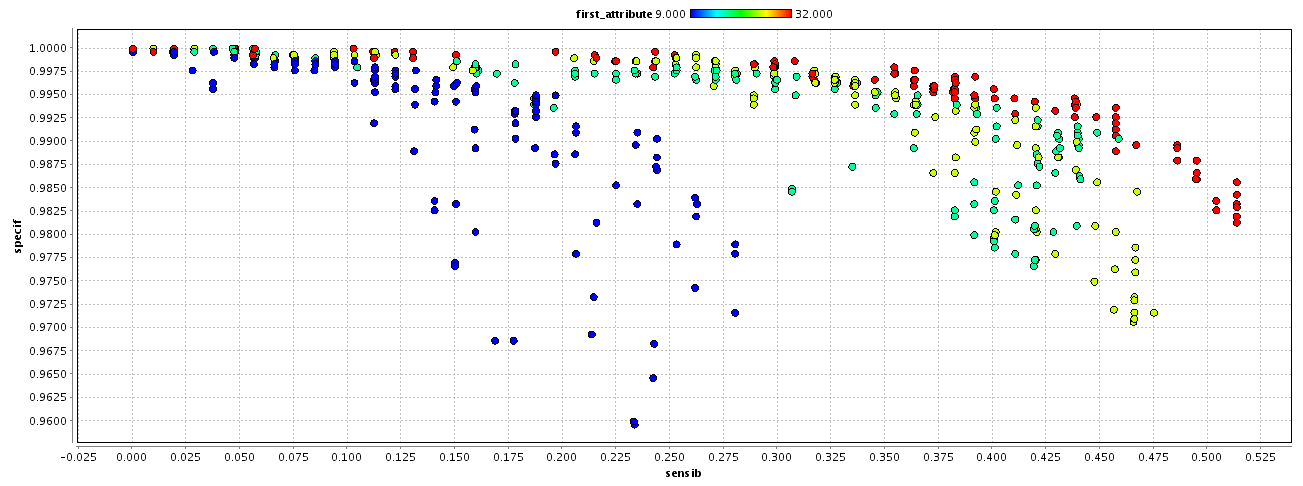
\includegraphics[width=14cm]{images/pareto_mod_LOR19.png}
 
{\small c) ET-LOR}
\vspace{0.5cm}

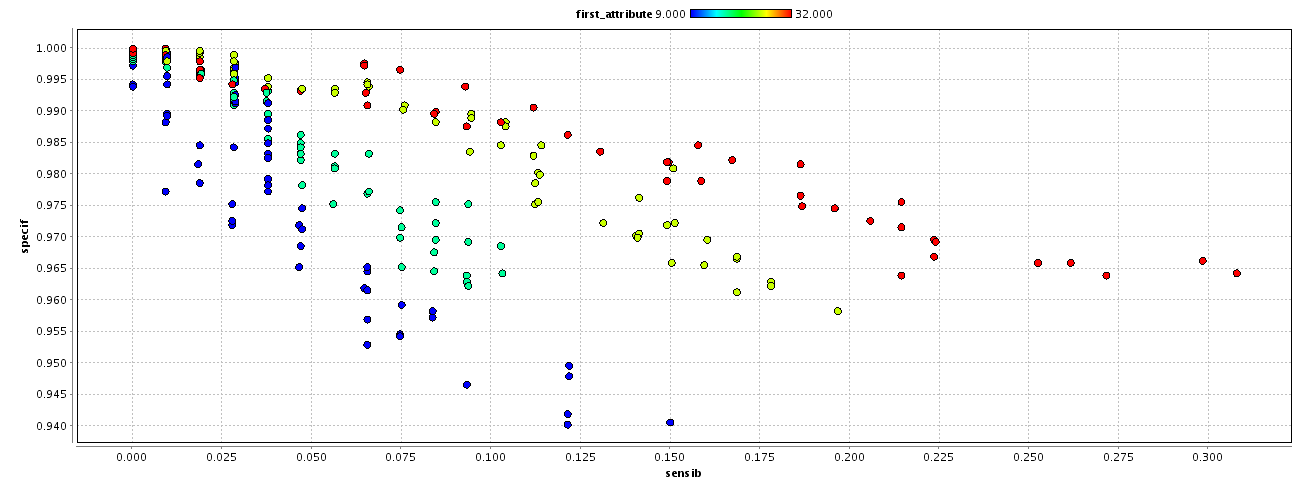
\includegraphics[width=14cm]{images/pareto_mod_NoCorr19.png}

{\small d) ET-NoCorr}

\end{center}
 \caption{\label{fig:paretoModalite19_2} Fronts de pareto des résultats de la recherche des meilleurs paramètres du classifieur pour les différentes modalités, avec 200 points négatifs par image. Pour chaque triplet de paramètres (C, $\gamma$, j), la sensibilité et la spécificité sont reportées sur le graphique. Le code couleur correspond à la valeur de j. c) représente la correction d'image pendant la reconstruction et d) le images non corrigées.}
\end{figure}



% Static : 857.6958985908936	0.001709975946676697	32.0	0.9790779315594078	0.6160173160173159	0.992
% LOR	 : 251.18864315095797	0.005323362023203629	32.0	0.969422309209811	0.5134199134199134	0.9856666666666667 
% NoCorr : 5411.6952654646375	0.001709975946676697	32.0	0.9417478291936561	0.30779220779220784	0.9643333333333333
% IM	 : 5411.6952654646375	5.49280271653059E-4	32.0	0.9826195691007659	0.6805194805194804	0.9933333333333334
\begin{figure}[h!]
\label{fig:paramsModFoie}
%	\begin{center}
		\begin{tabular}{c| c c c c c}
  \hline
  a	& Base Statique	& Base IM	& Base LOR	& Base NoCorr	\\
  \hline
 C 	& 858		& 5412		& 251		& 5412		\\
\hline
$\gamma$& 0.002		& 0.00055	& 0.0053	& 0.0017	\\
\hline
j	& 4		& 4		& 4		& 4		\\
\hline
\hline
Sensibilité& 0.62	& 0.68		& 0.51		& 0.31	\\
\hline
Spécificité& 0.99	& 0.99		& 0.99		& 0.96		\\
\hline
Précision& 0.98		& 0.98		& 0.97		& 0.94		\\
\hline
 		\end{tabular}

%	\end{center}
\caption{Paramètres sélectionnés pour l'optimisation des performances du Foie. Sont indiqués pour chaque base le triplet de paramètres sélectionné ainsi que sa position sur le front de pareto.}
\end{figure}
